\usepackage{amsmath}


\chapter{Reinforcement Learning}
In this chapter I will briefly explain the key concepts and methods of reinforcement learning that allow our model
learn the game of Schafkopf.
For this we will explain neural networks, their components and internal mechanisms, the reinforcement learning approach,
Proximal Policy Optimisation, which is the training algorithm used in our experiments.


\section{Neural Networks}
A \textbf{Neural Network (NN)} is an attempt to imitate the complex behaviour of the human brain that
enables us as humans to learn complex skills.
The human brain consists of billions of neurons, the basic building block inside the nervous system, that are
interconnected to form large networks, capable of processing an input signal,for example a visual stimulus, into an
output.\\

\subsection{Artificial Neuron}
To imitate this we define an artificial neuron, with the goal of creating a type of switch to process an input signal
to an output, which could again be connected to further neuron.
To do so, we give the artificial neuron an input, a weight associated with that input,an activation function and an
output.
A neuron may have multiple inputs as well as outputs and the connection between the output of one neuron to the input
of another neuron is called an edge, which in turn may have their own weights.
The output signal is calculated by passing the sum of all weighted input signals through the activation function and
can be express by the following formula:
\newline
\begin{center}
    \begin{math}
        \boxed{
            \begin{aligned}
                &\textrm{Let } k\textrm{ be the neuron }k,&\\
                &\textrm{let } n \textrm{ be the number of inputs }x,&\\
                &\textrm{let } w \textrm{ be the weight,}&\\
                &\textrm{and let }\phi \textrm{ be the activation function}&\\
                &y\textsubscript{k} = \phi (\sum_{i=0}^n w\textsubscript{kn}x\textsubscript{n})
            \end{aligned}}
        \caption{Formula to calcualate neuron output }
        \label{neuronactivation}
    \end{math}
\end{center}
There are a number of possible activation functions that can be used, but for our purpose we will look at
\textbf{Rectified Linear Unit (RELU)} and the \textbf{Softmax}.\\
\textbf{ReLU} is a simple activation function that forwards the input, if its positive, otherwise zero.
The \textbf{ReLU} function is formulated using:

\begin{center}
    \begin{math}
        \boxed{
            \begin{aligned}
                &\textrm{Let } x \textrm{ be the input of a \textbf{ReLU}}\\
                &f(x) = max(0,x)
            \end{aligned}
        }
        \caption{Definition of \textbf{ReLU} activation function}
        \label{activationRelu}
    \end{math}
\end{center}
\newline
Now that we defined a neuron, we can use multiple neurons to form a layer, which in turn can be connected in sequence
to form a \textbf{NN}.
The minimal architecture of a network consists of three layers, whereas the middle layers are named hidden layers:
\[\text{Input layer}\Rightarrow\text{Hidden layer}\Rightarrow\text{Output layer}\]
\newline
Between adjacent layers, every neuron's input is connected to the outputs of every neuron in the previous layer and
vice versa for the following layer.
See Fig. \ref{fig:architecture} for an example.
\newline

\begin{figure}[]
    \centering
    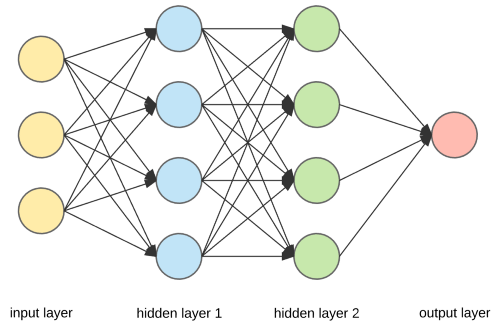
\includegraphics[scale=0.5,]{neuralnetlayer}
    \caption{Example architecture of a neural network with input,2 hidden and output layers}
    \label{fig:architecture}
\end{figure}
This kind of architecture is called \textbf{feed forward NN}, due to the process of passing an input linearly through
the network to the output, and will be used exclusively in our experiments.\\

\subsection{}
Initially any network is initialised with randomised weights
Learning


\section{Actor-Critic}


\section{Proximal Policy Optimisation}


\section{Self Play Learning}
